\documentclass[10pt,cn]{elegantbook}
\usepackage[utf8]{inputenc}
\usepackage[T1]{fontenc}
\usepackage{tgtermes}
\usepackage{amsmath}
\usepackage{amsfonts}
\usepackage{amssymb}
\usepackage{stmaryrd}
\usepackage{hyperref}
\hypersetup{colorlinks=true, linkcolor=blue, filecolor=magenta, urlcolor=cyan,}
\urlstyle{same}
\usepackage{graphicx}
\usepackage[export]{adjustbox}
\usepackage{mdframed}
\usepackage{booktabs,array,multirow}
\usepackage{esint}
\usepackage{xeCJK}
%\usepackage{adjustbox}
\usepackage[export]{adjustbox}
%\graphicspath{ {./images/} }

\usepackage{ulem}
\usepackage{hyperref}%目录跳转

\usepackage{fontspec} % 用于处理字体


\usepackage{circuitikz}

%\usepackage{fancyhdr}   % 导入 fancyhdr 包,用于定制页眉和页脚
%\usepackage{datetime}   % 导入 datetime 包,用于格式化日期


\usepackage{graphicx}   % 导入 graphicx 包,以便插入图片

\usepackage{tikz,tkz-euclide}


\usepackage{comment}

%\fancyhead[L]{20240722} % 左侧页眉
%\fancyhead[R]{\mydate\today} % 右侧页眉,显示当前日期,格式为“日 月 年”

\title{HappaPhysicsNotes}
\subtitle{物理笔记}
\author{OyamaHappa}
\date{\today}
\version{20240803125929}
\extrainfo{孔明是我的理想,商鞅是我的下场}
\logo{logo.jpg}
\cover{cover.jpg}



% 本文档命令
\usepackage{array}
\usepackage{mathdots}
\newcommand{\ccr}[1]{\makecell{{\color{#1}\rule{1cm}{1cm}}}}
% 修改目录深度
\setcounter{tocdepth}{3}

\everymath{\displaystyle}%用行间公式(displaystyle)的格式排版所有的行内公式


%\usepackage{verbatim}%在codeshow中已引用
\usepackage{tikz,tkz-euclide}
\usepackage{amsmath}
\usepackage{pgfplots}
%\usepackage{codeshow}%codeshow:为了在codeshow环境中,引用代码,并生成图形。

\usepackage{graphicx}
%\usepackage{subfigure}

\usepackage{breqn}%breqn 宏包主要提供了 dmath 和 dmath* 等几个环境,产生可以自动折行的显示公式。
\usepackage{longtable}%长表格,多页可以自动处理。

%【参与编译的文件列表。】
%\includeonly{preface,chapter01,chapter02,chapter03,chapter04,chapter05}%,%【参与编译的文件列表。】




\usepackage{amsmath}
\usepackage{amsfonts}
\usepackage{amssymb}
\usepackage{stmaryrd}
\usepackage{hyperref}
\hypersetup{colorlinks=true, linkcolor=blue, filecolor=magenta, urlcolor=cyan,}
\urlstyle{same}
\usepackage{graphicx}
\usepackage[export]{adjustbox}
\usepackage{mdframed}
\usepackage{booktabs,array,multirow}
\usepackage{esint}
\usepackage{xeCJK}
\usepackage{adjustbox}
\newcommand{\HRule}{\begin{center}\rule{0.5\linewidth}{0.2mm}\end{center}}
%\graphicspath{ {./images/} }
\usepackage{amsmath}
\usepackage{pifont}

\newcounter{num}

\usepackage[version=4]{mhchem}

\begin{document}
	
	\begin{titlepage}
		\begin{center}
			\vspace*{3cm}
			
			{\Large \textbf{HappaNotesBooks} }
			
			{\Large(试 用)}
			
			\vspace{1cm}
			
			{\Huge 物 \qquad 理}
			
			\vspace{0.5cm}
			
			
			
			
			
			
			\vspace{1cm}
			
			OyamaHappa
			
			
			\vspace{5cm}
			电学
			
			
			\vfill
			
			相逢即是下山时
			
			
			
		\end{center}
	\end{titlepage}
	
	%	\maketitle
	
	\tableofcontents
	%\listofchanges
	
	\mainmatter


\part{静电场中的能量}
\chapter{电容器}

\textit{任何两个彼此绝缘而又互相靠近的导体,都可
以看成是一个电容器}.这两个导体就是电容器的两个极,两
块正对的平行金属板,它们相隔很近而且彼此绝缘,就组成一
个最简单的电容器,叫做平行板电容器.

\textbf{额定电压 印着}

\textit{击穿电压}
 \section{电容}

 电容器带电的时候,它的两极之间产生电势差.实
 验证明,对任何一个电容器来说,两极间的电势差都随所带电
 量的增加而增加,而且电量跟电势差成正比,它们的比值是一
 个恒量,不同的电容器,这个比值一般是不同的.可见,这个
 比值表征了电容器的特性.\textit{电容器所带的电量跟它的两极间
 	的电势差的比值,叫做电容器的电容}.如果用$Q$表示电容器
 所带的电量,用$U$表示它的两极间的电势差,用$C$表示它的电
 容,那么,
 \[C=\frac{Q}{U} \]

 在国际单位制里,电容的单位是法拉,简称法,国际符号
 是F.一个电容器,如果带1库的电量时两极间的电势差是
 1伏,这个电容器的电容就是1法.
 \[1{\rm F}=1{\rm C}/{\rm V}\]
 
 法拉这个单位太大,实际上常用较小的单位:微法($\mu$F)
 和皮法(pF).它们间的换算关系是:
 \[1{\rm F}=10^6\mu{\rm F}=10^{12}{\rm pF}\]
 
 无线电收音机里常用的电容器,电容从几个皮法到几十
 个微法的都有.
  \subsection{决定式}


 	由于我们的知识不足,现在还不能从理论上进一步讨论
 上面的实验结果,可以指出:对于一个平行板电容器,如果两
 板的正对面积为$S$,两板的距离为$d$,两板间充满介电常数为
 $\varepsilon$的电介质,那么,它的电容可以用下式来表示.
 \[C=\dfrac{\varepsilon  S}{4\pi kd} \]
 
 k静电常数
 
 d板间距
 
 式中$S$用${\rm m^2}$作单位,$d$用${\rm m}$作单位,静电力恒量$k=9 \times 10^9{\rm N}\cdot {\rm m^2}/{\rm C^2}$
 ,算出的$C$以法为单位.可以看出,\textit{平行板电容器
 	的电容,跟介电常数成正比,跟正对面积成正比,跟极板的距
 	离成反比}.这跟上面的实验结果是一致的.
 
  \section{特点}

  \[E=\dfrac{U}{d}\]
C与	Q{} U无关{} 只与$\varepsilon s d$有关  
 \section{动态变化}
 
   \subsection{有源}
   
    \subsubsection{U不变}
    
    \begin{circuitikz}
    	\draw
    	(0,0) to[short, -*] (3,0) % 从电源到电容器左侧
    	(3,0) to[C] (3,-2) % 电容器
    	(3,-2) to[short, -*] (0,-2) % 电容器到电源下方
    	(0,-2) to[battery1] (0,0); % 电源
    \end{circuitikz}
    \[C=\dfrac{Q}{U}=\dfrac{\varepsilon  S}{4\pi kd}\]

        \subsubsection{下板下移}~{}\\

\begin{comment}

	\begin{circuitikz}
		\draw
		% 从(0,0)开始绘制,至(2,0)绘制一个电池(电源),带正负极
		(2,0) to[battery1] (0,0)
		
		% 从电源的右侧端点(2,0)到电容器左侧端点(4,0)绘制一条短路线,并在电容器左侧端点标记节点
		(2,0) to[short, -*] (4,0)
		% 在电容器上板中点标记一个点A
	%	node at (4,0) [above] {A};
		% 从电容器左侧端点(4,0)到电容器右侧端点(4,-2)绘制一个电容器
		(4,0) to[C] (4,-2)
		
		% 在电容器右侧端点(4,-2)绘制接地点符号
		(4,-2) node[ground] {}
		
		% 从电容器右侧端点(4,-2)绘制一条短路线到电源负极端点(0,-2)
		(4,-2) to[short, -*] (0,-2)
		
		% 从电源负极端点(0,-2)到电源左侧端点(0,0)绘制一条短路线
		(0,-2) to[short, -*] (0,0)
		
		% 在电容器中间点标记一个点P
		node[circ] at (4,-1) {P}; % 标记点
		
		% 在电容器上板中点标记一个点A
	%	node[circ] at (4,0) {};
	%	node at (4,0.25) {A}; % 标记点
		% 在电容器上板中点标记一个点A

		(4,0) node[circ, label=above:A] {};
	\end{circuitikz}
\end{comment}
    	\begin{center}
    	\includegraphics[max width=0.3\textwidth]{image/20240608-2.jpg}
    \end{center}
    
   $$d\uparrow c \downarrow Q\downarrow $$
    
    $$E=\dfrac{U_{AP}}{d_{AP}}=\dfrac{{\varphi}_{A}-{\varphi}_{B}}{d_{AP}}$$
    
    	$$    
    \left.
    \begin{aligned}
          E=\dfrac{U}{d\uparrow} \Rightarrow E \downarrow \\
    	\\
    	U_{AO}(\text{不变})={\varphi}_{A}-{\varphi}_{O} \Rightarrow {\varphi}_{A}\text{不变}
    \end{aligned}
    \right\}
    \Rightarrow ({\varphi}_{A}-{\varphi}_{B})\downarrow \Rightarrow \uwave{ {\varphi}_{B}\uparrow}
    $$
    
      \subsection{无源}
      
      \subsubsection{Q不变}
      
     $$C=\dfrac{Q}{U}=\dfrac{\varepsilon  S}{4\pi kd}$$
      
      $$d\uparrow, C\downarrow, U\uparrow$$
      
      $C=\dfrac{Q}{U}\Rightarrow U=\dfrac{Q}{C}$
      
      $$E=\dfrac{U}{d}=\dfrac{Q}{c d}=\dfrac{4{\pi}kQ}{{\varepsilon}s}\Rightarrow\text{不变}$$
      
      \subsubsection{下板下移}
      
      
  \begin{circuitikz}
  	\draw
  	% 从电容器左侧端点(0,0)到电容器右侧端点(0,-2)绘制一个电容器
  	(0,0) to[C] (0,-2)
  	
  	% 在电容器右侧端点(0,-2)绘制接地点符号
  	(0,-2) node[ground] {}
  	
  	% 在电容器中间点标记一个点P
  	node[circ] at (0,-1) {P}; % 标记点
  	
  \end{circuitikz}
      
      
      $$    
      \left.
      \begin{aligned}
      	E(\text{不变})=\dfrac{U_{PO}}{d_{PO}}=\dfrac{{\varphi}_{P}-{\varphi}_{O}}{d_{PO}} \\
      	\\
      	{\varphi}_{o}=0,d_{po}\uparrow
      \end{aligned}
      \right\}
      \Rightarrow \uwave{{\varphi}_{P}\uparrow}
      $$
      
   \section{电容器的连接}
   
   实际使用电容器时,有时会遇到电容器的电容不够或耐
   压能力不够,这就需要把几个电容器连接起来使用,连接的基
   本方法有串联和并联两种.
   \subsection{电容器的串联}
   
   把几个电容器的极板首尾相接,连成一
   串,这就是电容器的串联,图6.40是三个电容器的串联,接
   上电压为$U$的电源后,两端极分别带电$+Q$和$-Q$.由于静
   电感应,中间各极所带的电量也等干$+Q$或$-Q$,所以串联时
   每个电容器带的电量都是$Q$.如果各个电容器的电容分别为
   $C_1$、$C_2$、$C_3$,电压分别为$U_1$、$U_2$、$U_3$,那么,
   \[ U_1=\frac{Q}{C_1},\qquad U_2=\frac{Q}{C_2},\qquad U_3=\frac{Q}{C_3}\]
   总电压$U$等于各个电容器上的电压之和,所以,
   \[U=U_1+U_2+U_3=Q(\frac{1}{C_1}+\frac{1}{C_2}+\frac{1}{C_3})\]
   设串联电容器的总电容为$C$,则$U=Q/C$,所以
   \[\frac{1}{C}=\frac{1}{C_1}+\frac{1}{C_2}+\frac{1}{C_3}\]
   这就是说,\textit{串联电容器的总电容的倒数等于各个电容器的电
   	容的倒数之和}.电容器串联之后,相当于增大了两极的距离,
   因此总电容小于每个电容器的电容.
   
   \begin{figure}[htp]\centering
   	\begin{circuitikz}[european]
   		\draw (0,0)--(0,2);
   		\draw (0,2)to [capacitor=$C_1$](2,2)to [capacitor=$C_2$](4,2)to [capacitor=$C_3$](6,2);
   		\draw (6,0)--(6,2);    
   		\draw (0,0) to [battery] (6,0)   ;
   		\node at (3,-.75){$U$};
   		
   		\foreach \x in {1,3,5}
   		{
   			\node at (\x,1.5)[left]{$+Q$};
   			\node at (\x,1.5)[right]{$-Q$};
   			
   		}
   		
   	\end{circuitikz}
   	
   	\caption{电容器的串联}
   \end{figure}
   
   
   
   \subsection{电容器的并联} 
   \begin{figure}[htp]\centering
   	\begin{circuitikz}[european]
   		\draw (0,0)--(6,0);
   		\draw (0,3)--(6,3);
   		\draw (0,3) to [C=$C_1$, *-*](0,0);
   		\draw (2,3) to [C=$C_2$, *-*](2,0);
   		\draw (4,3) to [C=$C_3$, *-*](4,0);
   		\foreach \x in {1,2,3}
   		{
   			\node at (2*\x-2-.5,1.7)[above]{$+Q_{\x}$};
   			\node at (2*\x-2-.5,1.3)[below]{$-Q_{\x}$};
   		}
   		\draw (6,3) to [battery] (6,0)   ;     
   		\node at (6.7,1.5){$U$};
   	\end{circuitikz}
   	
   	\caption{电容器的并联}
   \end{figure}	
   
   把几个电容器的正极连在一起,负极也
   连在一起,这就是电容器的并联.图6.41是三个电容器的并
   联.接上电压为$U$的电源后,每个电容器的电压都是$U$.如
   果各个电容器的电容分别为$C_1$、$C_2$、$C_3$,所带电量分别为$Q_1$、$Q_2$、$Q_3$,那么,
   \[Q_1=C_1U,\qquad Q_2=C_2U,\qquad Q_3=C_3U\]
   电器组贮存的总电量$Q$等于各个电容器所带电量之和,
   所以,
   \[Q=Q_1+Q_2+Q_3=(C_1+C_2+C_3)U\]
   设并联电容器的总电容为$C$,则$Q=CU$,所以,
   \[C=C_1+C_2+C_3\]
   这就是说,\textit{并联电容器的总电容等于各个电容器的电容之和}.
   电容器并联之后,相当于增大了两极的面积,因此总电容大于
   每个电容器的电容.
   
   电容器串联后,电容减小了,但耐压能力提高了,所以要
   承受较高的电压,可以把电容器串联起来;电容器并联后,电
   容增大了,耐压能力没有提高,所以在需要大电容时,可把
   电容器并联起来.
      
      \part{电路及其应用}
      
      \chapter{恒稳电流}
      
      \section{电流}
      
      \subsection{形成电流}
      
      \ding{172}自由电荷(e,正负离子)
      
       \ding{173}两端电压(电势差)
       
       \subsection{电流强度}
       
       电流有强弱的不同,电流的强弱用电流强度来表示.\textit{通过导体横截面的电量跟通过这些电量所用的时间的比值,叫做\textbf{电流强度}}.如果时间$t$内通过导体横截面的电量为$q$,那么电流强度
       \[I=\frac{q}{t} \]
       在国际单位制中,电流强度的单位是\textbf{安培},简称安,国际
       符号是A,如果在1秒内通过导体横截面的电量是1库仑,导体中的电流强度就是1安培,常用的电流强度的单位还有毫安(mA)、微安($\mu$A).
       \[\begin{split}
       	1{\rm mA}&= 10^{-3}{\rm A}\\
       	1{\rm \mu A}&=10^{-6}{\rm A}
       \end{split}\]
       
       导体中的电流既可以是正电荷的移动,也可以是负电荷的移动,还可以是正、负电荷沿相反方向的移动.因为负电荷的移动可看作正电荷沿相反方向的移动,所以为了便于分析问题,习惯上规定正电荷的移动方向为电流的方向,这样,在金属导体中电流的方向就与自由电子移动的方向相反.在电解液中,电流的方向与正离子移动的方向相同,与负离子移动的方向相反.我们知道,正电荷在电场力的作用下是从电势高处向电势低处移动,所以导体中电流的方向是从电势高的一端流向电势低的一端,电源上电势高的电极叫正极,电势
       低的电极叫负极,所以在电源外部的电路中,电流的方向是从电源的正极流向负极.
       
       电路中,如果电流的方向不随时间而改变,这样的电流叫做\textbf{直流电};如果电流的方向和大小都不随时间而改变,这样的电流叫做\textbf{稳恒电流},这一章我们研究稳恒电流.
       
       \textbf{\textit{比值定义法}},\dotuline{标量}但有方向
       
       \subsection{环形电流}
       
       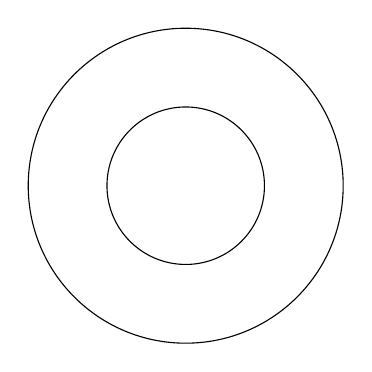
\begin{tikzpicture}
       	% 画第一个圆,半径为2
       	\draw (0,0) circle (1);
       	% 画第二个圆,半径为4
       	\draw (0,0) circle (2);
       \end{tikzpicture}
       
       $$I=\dfrac{Q}{t}=\dfrac{e}{T}=\dfrac{e \omega}{2\pi}$$
       
       \subsection{电解槽}
       

    \begin{center}
    \includegraphics[max width=0.3\textwidth]{image/20240708-2.jpg}
    \end{center}
    
     \subsection{决定式}
     
      \begin{center}
     	\includegraphics[max width=0.3\textwidth]{image/20240708-3.jpg}
     \end{center}
     
    v匀速
    
    S导体横截面积
    
    n单位体积内电子的个数
    
    $I=\dfrac{Q}{t}=\dfrac{v\cdot t\cdot s\cdot n\cdot q}{t}=nqav$
    
    	\begin{center}
    	\framebox{\begin{minipage}{12em}
    			\begin{gather*}
    				I=nqav
    			\end{gather*}
    	\end{minipage}}
    \end{center}
    
    \subsection{速度}
    
    电子定向移动$10^{-5}$m/s
    
    电子热运动$10^{-5}$m/s
    
    电流形式$c$
    
    \section{电动势}
    
    电源:非静电力(化学作用)
    
    \textit{电动势反映了电源的一种特性,它在数值上等于电路中通过1库仑电量时电源所提供的电能}.电源提供的电能是由其形式的能转化来的.例如,在化学电池中电能是由化学能转化来的,在发电机中电能是由机械能转化来的.从本质上来说,各种电源都是把其他形式的能转化为电能的装置.电动势越大,表明电源把其他形式的能转化为电能的本领越大.
    
    $$E=\dfrac{W}{q}$$
    
    单位:V,比值定义法
    
    \subsection{物理意义}
    
    电源把其他形式的能转换成电能的本领
    
    \dotuline{标量}但有方向,\textit{电源内从负$\rightarrow$正}
    
     \section{内阻}
     
     \begin{circuitikz}[european, scale=.8]
     %	european: 这个选项指定了使用欧洲风格的电气符号,这些符号与美国风格的符号略有不同。例如,电阻和电容的符号在这两个风格中有所不同。
     %	scale=.8: 这个选项缩放整个电路图到原来的 80%,即缩小到 80%。这在需要调整图表大小以适应文档布局时非常有用。
     \draw
     % 从(0,0)开始绘制一个电源(电池),带正负极
     (0,0) to[battery1] (2,0)
     
     % 从电源右端点(2,0)到电阻左端点(4,0)绘制一条短路线
     (2,0) to[short] (3,0)
     
     % 从电阻左端点(4,0)到电阻右端点(6,0)绘制一个电阻
     (3,0) to[R=$R$, *-*] (5,0)
     
      (5,0) to[short] (7,0)
     % 从电阻右端点(6,0)绘制一条短路线回到电源负极端点(0,0)
     %(6,0) to[short] (6,-2) to[short] (0,-2) to[short] (0,0)
     ;
     \end{circuitikz}
     
     当电路为短路时电源两端在电压在数值上=电动势
     
      \section{电池容量}
      
      放电时放出的总电量
      
      $$Q=It$$
      
      单位:Ah
      
      \subsection{做的功}
      
      $$W=UIt$$
      
      \section{电阻}
      
      在导体两端加上电压,导体中就有电流,导体中电流的强弱跟加在导体两端的电压有什么关系呢?德国物理学家欧姆(1787—1854)通过实验研究,对导体中电流与电压的关系
      得出了如下的结论:\textit{通过导体的电流跟加在导体两端的电压成正比},即$I\propto U$.通常把这个关系写作
      \[\frac{U}{I}=R\]
      
      式中$R$是电压与电流的比值,实验表明,对同一根导线来说,不管电压和电流的大小念样变化,比值$R$都是相同的,对于不同的导线,$R$的数值一般是不同的.这表明,$R$是一个跟导体本身有关的量,导线的$R$越大,在同一电压下,通过它的电流就越小.可见,比值$R$反映出导线对电流的阻碍作用,我们把它叫做导体的\textbf{电阻}.
      
      上面的公式可写成
      \[I=\frac{U}{R}\]
      这个公式表示\textbf{导体中的电流强度跟导体两端的电压成正比,跟导体的电阻成反比}.这就是我们在初中学过的\textbf{欧姆定律}.
      
      根据欧姆定律可以规定电阻的单位,电阻的单位是\textbf{欧姆},简称欧,国际符号是$\Omega$. 它是这样规定的:如果在某段导线两端加上1伏特电压,通过它的电流强度是1安培,这段导线的电阻就是1欧姆.
      \[1\Omega=\frac{1{\rm V}}{1{\rm A}} \]
      
      1常用的电阻单位还有千欧(k$\Omega$)和兆欧(M$\Omega$).
      \[\begin{split}
      	1{\rm k}\Omega&= 10^{3}\Omega\\
      	1{\rm M}\Omega&=10^{6}\Omega
      \end{split}\]
      
   %   应该注意的是,欧姆定律是在金属导电的基础上总结出来的,对于其他导体是否适用,还要经过实验的检验.实验结果是,除金属外,欧姆定律对电解液导电也适用,但对气体导电就不适用了.
      
      
      $$R=\dfrac{U}{I}$$
      
      \textit{比值定义法}
      
      \subsection{决定式}
      
      \textit{导线的电阻跟它的长度成正比,跟它的横截面积成反比}.这就是\textbf{电阻定律},用公式来表示可以写作
      \begin{center}
      	\framebox{\begin{minipage}{12em}
      			\begin{gather*}
      				  R=\rho\frac{\ell}{S}
      			\end{gather*}
      	\end{minipage}}
      \end{center}
    
     
      式中的比例系数$\rho$跟导体的材料有关系.在一定的温度
      下,对同一种材料$\rho$是一个常数,对不同的材料$\rho$的数值不同,横截面积和长度都相等的不同材料的导线.$\rho$越大的电阻越大,$\rho$越小的电阻越小.可见,$\rho$是一个反映材料导电性好坏的物理量,叫做材料的\textbf{电阻率}.
      
      $T\uparrow \rho \uparrow$
      
      把上面的公式改写作
      \[\rho=R\frac{S}{\ell}\]
      式中$\ell=1{\rm m}$,$S=1{\rm m^2}$时,$\rho$的数值等于$R$.可见,材料的电阻率在数值上等于这种材料制成的长1${\rm m}$、横截面积1${\rm m}^2$的导体的电阻.
      
      根据上式,可以确定电阻率$\rho$的单位,$R$的单位是$\Omega$,$S$的单位是${\rm m^2}$,$\ell$的单位是m.所以$\rho$的单位是欧姆·米,简称欧·米,国际符号是$\Omega\cdot {\rm m}$.
      
      $U=IR=nqsv\cdot \rho \dfrac{L}{S}=nev\rho L$
      
         \begin{center}
      	\framebox{\begin{minipage}{12em}
      			\begin{gather*}
      			E=\dfrac{U}{L}=nev\rho
      			\end{gather*}
      	\end{minipage}}
      \end{center}
\subsection{闭合电路欧姆定律}

\subsubsection{电动势}
\subsubsection{电路}

内电路(内阻)纯电阻

外电路 用电器

\subsubsection{表达式}

\paragraph*{电流}

\begin{center}
	\framebox{\begin{minipage}{12em}
			\begin{gather*}
				I_{\text{干}}=\dfrac{E}{R+r}
			\end{gather*}
	\end{minipage}}
\end{center}

$$\text{{\large \textbf{\textit{纯电阻}}}}$$


\paragraph*{电压}

\begin{center}
	\framebox{\begin{minipage}{12em}
			\begin{gather*}
				E_{\text{路端电压}}=U_{\text{路}}+Ir
			\end{gather*}
	\end{minipage}}
\end{center}

$$\text{{\large \textbf{\textit{通用}}}}$$



\begin{tikzpicture}
	% 画坐标轴,x 轴和 y 轴
	\draw[->] (0,0) -- (5,0) node[right] {$U_{\text{路}}$}; % 画 x 轴,箭头指向右,标注 U路
	\draw[->] (0,0) -- (0,5) node[above] {$I$}; % 画 y 轴,箭头指向上,标注 I
	
	% 画一次函数 y = -x + 4 的图像,只显示第一象限部分
	% domain=0:4 表示 x 从 0 到 4,4-\x 表示 y 的值,node[right] 用于在右侧标注函数公式
	\draw[domain=0:4] plot(\x, {4-\x}) ;
	
	% 标记直线在 y 轴上的交点 (0,4)
	% \fill 命令用于绘制一个实心圆点,(0,4) 是点的坐标,circle (2pt) 表示点的半径为 2pt,node[left] 用于在左侧标注点的坐标
%	\fill (0,4) circle (2pt) node[left] {$(0,4)$};
	
	% 标记直线在 x 轴上的交点 (4,0)
	\fill (4,0) circle (2pt) node[below] {$I=\frac{E}{r}$};
	
	\node at (4,-1) {$\text{短路}$};
	
	 % 在右上方标注函数公式
	\node[anchor=south west] at (2,2) {$k=-r$};
\end{tikzpicture}


$$U=-rI+E$$

\section{电功率}

\subsection{纯电阻}

$$P=UI=I^{2}R=\dfrac{U^{2}}{R}$$

\subsection{非纯电阻(电动机)}

$$P=UI$$

$
\left\{
\begin{aligned}
	P_{\text{热}}=I^{2}R \\
	\\
	P_{\text{机}}=UI-I^{2}R
\end{aligned}
\right.
$

$UI>I^{2}R$

$$I<\dfrac{U}{R}$$
\subsubsection{堵转}

$P_{\text{机}=0}\Rightarrow$纯电阻

\section{电源模型}

$$P_{\text{总}}=EI$$

$$P_{\text{内}}=I^{2}r$$

$$P_{\text{外}}=P_{\text{输出}}=EI-I^{2}r=U_{\text{路}}I$$

\textbf{\textit{{\Large 当$R=r$时,$P_{\text{输出}}$最大}}}

\begin{tikzpicture}
	\begin{axis}[
		domain=0:10, % 定义 x 轴的范围
		samples=100, % 样本数,决定图像的平滑程度
		xlabel={$R$}, % x 轴标签
		ylabel={$P_{\text{输出}}$}, % y 轴标签
		axis lines=middle, % 坐标轴穿过原点
	%	xtick={$r$}, % x 轴刻度
	%	ytick={3.125}, % y 轴刻度
	 xtick=\empty, % 去掉 x 轴刻度
	ytick=\empty, % 去掉 y 轴刻度
		yticklabel style={ /pgf/number format/fixed }, % 固定 y 轴刻度标签格式
		enlargelimits=true, % 增加坐标轴范围
		clip=false % 允许标注超出坐标轴范围
		]
		% 绘制功率曲线,E=5, r=2
		\addplot[
		blue,
		thick
		]{5 * (5 / (x + 2)) - (5 / (x + 2))^2 * 2};
		
		% 标记最大功率点 P_max
		\draw[dashed] (axis cs:2,0) -- (axis cs:2,3.125); % 垂直虚线
	%	\draw[dashed] (axis cs:0,3.125) -- (axis cs:2,3.125); % 水平虚线
		\node[anchor=south west] at (axis cs:2,3.125) {$P_{\text{max}}$}; % 标注 P_max
		
		% 标记 P_max 点
		\fill (axis cs:2,3.125) circle (2pt);
	% 标记内阻 r
	\node[below] at (axis cs:2,0) {$r$};
	\end{axis}
\end{tikzpicture}

\subsection{例}

 \begin{circuitikz}[european, scale=.8]
	%	european: 这个选项指定了使用欧洲风格的电气符号,这些符号与美国风格的符号略有不同。例如,电阻和电容的符号在这两个风格中有所不同。
	%	scale=.8: 这个选项缩放整个电路图到原来的 80%,即缩小到 80%。这在需要调整图表大小以适应文档布局时非常有用。
	\draw

	(2,0) to[battery1] (4,0)
	
	(0,0) to[short] (2,0)
	
    (0,0) to[short] (0,2)

    (0,2) to[short] (1,2)
 
	(1,2) to[R=$R_{0}$, *-*] (2,2)
	
	
	(2,2) to[short](3,2)
	 % 滑动变阻器
	(3,2) to[variable resistor, l=$Rp$] (5,2)
	
	(5,2) to[short](6,2)
	
	(6,2) to[short](6,0)
	
	(4,0) to[short] (6,0)


	;
\end{circuitikz}

\subsubsection*{\ding{172}$P_{R_{0}}$最大}

$$P_{R_{0}}=I^{2}R$$

\subsubsection*{\ding{173}$P_{\text{输出}}$最大}

$$R_{0}+Rp=r$$

\subsubsection*{\ding{174}$P_{Rp}$最大}

$$Rp=R_{0}+r$$

\subsection{效率}

$${\eta}_{\text{纯电阻}}=\dfrac{P_{\text{输}}}{P_{\text{总}}}=\dfrac{I^{2}R}{I^{2}(R+r)}=\dfrac{R}{R+r}=\dfrac{1}{1+\dfrac{r}{R}}$$

{\Large $\Rightarrow R\uparrow,\eta \uparrow$}

\section{P-I图}

$$P_{\text{总}}=EI$$

$$P_{\text{内}}=I^{2}r$$

$$P_{\text{外}}=EI-I^{2}r$$

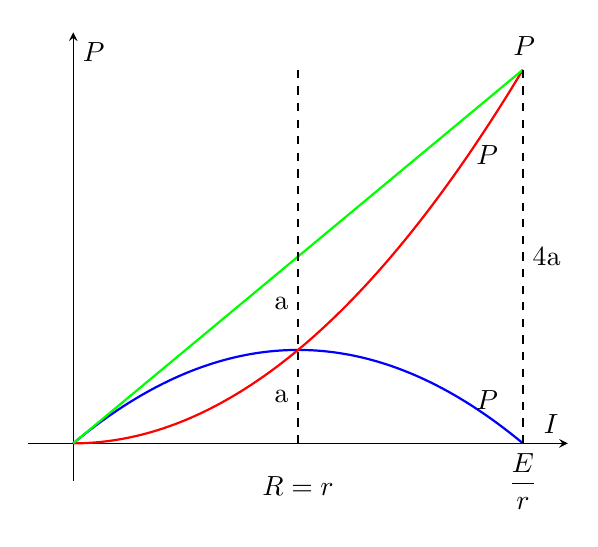
\begin{tikzpicture}
	\begin{axis}[
		domain=0:4, % 定义 x 轴的范围
		ymax=8, % 设置 y 轴最大值
		samples=100, % 样本数,决定图像的平滑程度
		xlabel={$I$}, % x 轴标签
		ylabel={$P$}, % y 轴标签
		axis lines=middle, % 坐标轴穿过原点
		xtick=\empty, % 去掉 x 轴刻度
		ytick=\empty, % 去掉 y 轴刻度
		yticklabel style={ /pgf/number format/fixed }, % 固定 y 轴刻度标签格式
		enlargelimits=true, % 增加坐标轴范围
		clip=false % 允许标注超出坐标轴范围
		]
		% 绘制 y = -0.5*x^2 + 2*x
		\addplot[
		blue,
		thick
		]{-0.5*x^2 + 2*x};
		
		% 绘制 y = 0.5*x^2
		\addplot[
		red,
		thick
		]{0.5*x^2};
		
		% 绘制 y = 2*x
		\addplot[
		green,
		thick
		]{2*x};
		
		% 绘制 x = 2 的竖线
		\addplot[
		dashed,
		black,
		thick
		] coordinates {(2,0) (2,8)};
		
		% 绘制 x = 4 的竖线
		\addplot[
		dashed,
		black,
		thick
		] coordinates {(4,0) (4,8)};
		
 % 在 x=2 下面标注 R=r
\node at (axis cs:2,-0.5) [anchor=north] {$R=r$};

% 在 (4,0) 处标注 \dfrac{E}{r}
\node at (axis cs:4,0) [anchor=north] {$\dfrac{E}{r}$};

\node at (axis cs:2,1) [anchor=east] {a};

\node at (axis cs:2,3) [anchor=east] {a};

\node at (axis cs:4,4) [anchor=west] {4a};

\node at (axis cs:4,8) [anchor=south] {$P_{\text{总}}$};

\node at (axis cs:3.5,6.125) [anchor=west] {$P_{\text{内}}$};

\node at (axis cs:3.5,0.875) [anchor=west] {$P_{\text{输出}}$};
	\end{axis}

\end{tikzpicture}

\textbf{\textit{{\LARGE 当$R=r$时,$P_{\text{外}}=P_{\text{内}}$且$P_{\text{外}}$最大}}}

\section{U-I图}

$$E=U_{\text{路}}+Ir$$

$$U_{\text{路}}=-rI+E$$

\begin{comment}


\begin{tikzpicture}
	\begin{axis}[
		domain=0:4, % 定义 x 轴的范围
		ymax=4, % 设置 y 轴最大值
		samples=100, % 样本数,决定图像的平滑程度
		xlabel={$I$}, % x 轴标签
		ylabel={$U$}, % y 轴标签
		axis lines=middle, % 坐标轴穿过原点
		xtick=\empty, % 去掉 x 轴刻度
		ytick=\empty, % 去掉 y 轴刻度
		yticklabel style={ /pgf/number format/fixed }, % 固定 y 轴刻度标签格式
		enlargelimits=true, % 增加坐标轴范围
		clip=false % 允许标注超出坐标轴范围
		]
		% 绘制 y = -0.5*x^2 + 2*x
		\addplot[
		blue,
		thick
		]{x};
		
		\addplot[
		red,
		thick
		]{-x+4};
		
		\node at (axis cs:0,4) [anchor=east] {$E$};
		
		\node at (axis cs:4,0) [anchor=north] {$\dfrac{E}{r}$};
	\end{axis}

\end{tikzpicture}

\end{comment}


\begin{center}
	\includegraphics[max width=0.5\textwidth]{image/20240910-2.jpg}
\end{center}


\section{电阻U-I}

\begin{tikzpicture}
	\begin{axis}[
		domain=0:4, % 定义 x 轴的范围
		ymax=16, % 设置 y 轴最大值
		samples=100, % 样本数,决定图像的平滑程度
		xlabel={$I$}, % x 轴标签
		ylabel={$U$}, % y 轴标签
		axis lines=middle, % 坐标轴穿过原点
		xtick=\empty, % 去掉 x 轴刻度
		ytick=\empty, % 去掉 y 轴刻度
		yticklabel style={ /pgf/number format/fixed }, % 固定 y 轴刻度标签格式
		enlargelimits=true, % 增加坐标轴范围
		clip=false % 允许标注超出坐标轴范围
		]
		% 绘制 y = x^2
		\addplot[
		blue,
		thick
		]{x^2};
		
		% 绘制 x = 3 的竖线
		\addplot[
		dashed,
		black,
		thick
		] coordinates {(3,0) (3,9)};
		
				\addplot[
		dashed,
		black,
		thick
		] coordinates {(0,9) (3,9)};
		
		
		% 在 x=3 下面标注 R=r
		\node at (axis cs:3,-0.5) [anchor=north] {$I_{1}$};
		
		% 在 (3,9) 处标注 \dfrac{E}{r}
		\node at (axis cs:0,9) [anchor=east] {$U_{1}$};
		
	\end{axis}
\end{tikzpicture}


\textbf{\textit{{\LARGE 切线斜率$\neq $阻值}}}

\textbf{\textit{{\LARGE 割线斜率= 阻值}}}

\section{变化量问题}

\textbf{\textit{{\Large 串反并同}}}

$Rp\Rightarrow U,I$

\begin{circuitikz}[european,>=latex, yscale=.8] % 开始电路图环境,设置为欧洲风格箭头,使用latex箭头样式,y轴缩放0.8倍
% 电池
\draw (4,0) to[battery1] (5,0); % 在(0,0)到(6,0)之间绘制一个电池,标记为V

% 主电路中的定制电阻
\draw   (2.5,0) to[R] (3.5,0); 

\draw (3.5,0) -- (4,0);


\draw  (6,0.5)  to[R] (6,1); 
% 并联部分的定制电阻
\draw (4,1) to[R] (5,1); 

% 并联部分的滑动变阻器
\draw (4,2) to[R] (5,2); 

% 滑动变阻器的箭头
\draw (6,1.5) -- (4.5,1.5); 
\draw[->] (4.5,1.5) -- (4.5,1); % 绘制箭头的箭头部分




\draw (5,0) -- (6,0);

\draw (6,0) -- (6,0.5);

\draw (2.5,0) -- (1,0);

\draw (1,0) -- (1,2);

\draw (1,1) -- (4,1);

\draw (1,2) -- (4,2);

\draw (5,2) -- (6,2);

\draw (6,2) -- (6,1);






\node at (4.5,2) [anchor=south] {$U_{1}$};
\node at (6,1) [anchor=west] {$U_{2}$};
\node at (2.5,0) [anchor=south] {$U_{3}$};

\node at (3,2) [anchor=south] {$A_{1}$};
\node at (3,1) [anchor=west] {$A_{2}$};

\end{circuitikz}



{\large $$|\varDelta U_{1}|>|\varDelta U_{2}|$$}

$|\varDelta U_{1}|(\text{变大})=|\varDelta U_{2}|(\text{变小})+|\varDelta U_{3}|(\text{变小})$


{\large $$|\varDelta I_{1}|<|\varDelta I_{2}|$$}

$|\varDelta I_{2}|(\text{变小})-|\varDelta I_{2}|(\text{变大})=|\varDelta I_{\text{干}}|(\text{变小})$

\section{$\dfrac{\varDelta U}{\varDelta I}$问题}

\begin{circuitikz}[european,>=latex, yscale=.8] % 开始电路图环境,设置为欧洲风格箭头,使用latex箭头样式,y轴缩放0.8倍
% 电池
\draw (1,0) to[battery1] (2,0); % 在(0,0)到(6,0)之间绘制一个电池,标记为V

% 主电路中的定制电阻
\draw   (0.5,2) to[R] (1.5,2); 

\draw  (2.5,2)  to[R] (3.5,2); 

% 滑动变阻器的箭头
\draw (2,2) -- (2,2.5); 
\draw (2,2.5) -- (1,2.5); 
\draw[->] (1,2.5) -- (1,2); % 绘制箭头的箭头部分


\draw (1,0) -- (0,0); 
\draw (0,0) -- (0,2);
\draw (0,2) -- (0.5,2);  
\draw (1.5,2) -- (2.5,2); 
\draw (3.5,2) -- (4,2);
\draw (4,2) -- (4,0);
\draw (4,0) -- (2,0);   



\node at (1,2.5) [anchor=south] {$U_{1}/I_{1}$};
\node at (1,1.5) [anchor=north] {$Rp$};

\node at (3,2.5) [anchor=south] {$U_{2}/I_{2}$};
\node at (3,1.5) [anchor=north] {$R_{0}$};
\end{circuitikz}

\subsection*{右拨}
$$E=U_{1}+I_{1}(r+R_{0})$$
$$\Rightarrow U_{1}=-(r+R_{0})I_{1}+E$$

{\Large $$\dfrac{U_{2}}{I_{2}}=R_{0}\Rightarrow\text{不变}$$}
	
	{\Large $$\dfrac{\varDelta U_{2}}{\varDelta I_{2}}=R_{0}\Rightarrow \text{不变}$$}
		
{\Large $$\dfrac{U_{1}}{I_{1}}=R_{p}\Rightarrow \uparrow$$}

{\LARGE $$|\dfrac{\varDelta U_{1}}{\varDelta I_{1}}|=r+R_{0}\Rightarrow \text{不变}$$}

\chapter{长度的测量}

\section{估读}

在最小分度值后再添一位

\subsection{何时估读}

最小分度值以1结尾

\section{游标卡尺}

      \begin{center}
	\includegraphics[max width=0.8\textwidth]{image/B62.jpg}
\end{center}


主尺读+副尺读数

主尺:副尺上0刻度线左侧的刻度

副尺:重合刻度$\times \dfrac{1mm}{\text{副尺刻度数}}$


\subsection{读数步骤}

1. 读取主尺上的“mm”数。(要注意主尺数字的单位为 \(\mathrm{{cm}}\) ,但读数时请读“mm”数)

2. 找出游标尺上“0”以后的第n条刻度线与主尺上的某条刻线对的最齐,读出游标尺的“mm”数。 游标尺读数方法如下:


\begin{center}
	\adjustbox{max width=\textwidth}{
		\begin{tabular}{|c|c|c|}
			\hline
			游标卡尺类型 & 游标尺“mm” & 游标尺“mm”数的形式 \\
			\hline
			10 分度 & n$\times$0.1 mm & \(0.\mathrm{x}\mathrm{\;{mm}}\) (最后一位数字可为 0\~9 中的任意一个整数) \\
			\hline
			20 分度 & n$\times$0.05 mm & 0.xx mm(最后一位数字只可能为 0、5 中的一个) \\
			\hline
			50 分度 & n$\times$0.02 mm & 0.xx mm(最后一位数字只可能为 0、2、4、6、8 中的一个) \\
			\hline
		\end{tabular}
	}
\end{center}

3. 待测长度 \(\mathrm{L} =\) “主尺 \(\mathrm{{mm}}\) 读数”+“游标尺 \(\mathrm{{mm}}\) ”数 (注意,游标卡尺读数不用估读哦);

4. 如有需要,讲读数换算成题意要求的单位。

\section{螺旋测微器}

      \begin{center}
	\includegraphics[max width=0.8\textwidth]{image/B64.jpg}
\end{center}

\subsection{读数}

1.读出固定刻度上的 mm 数,注意固定刻度线上的半毫米刻度线是否露出,未露出时为整数, 露出时要加 \({0.5}\mathrm{\;{mm}}\) ,如图为 \(7\mathrm{\;{mm}}\) ;

2.读出旋转刻度数值,要注意最后的估读数字,其形式一定为 \(0.\mathrm{{xxx}}\mathrm{{mm}}\) ,如图为

\[
{29.5} \times {0.01} = {0.295}\mathrm{\;{mm}}\text{;}
\]

3.待测长度=“固定刻度的 mm 数”+“可动刻度的 mm 数”,如图 L=7mm+0.295mm=7.295mm;

读数公式:

测量值=固定刻度值+固定刻度的中心水平线与可动刻度对齐的位置的读数$\times$0.01mm

\chapter{电路实验}

{\large 电流表分压}

{\large 电压表分流}

\textbf{\textit{适用于$R_{A}R_{V}$约为$\Rightarrow$}}
  $$    
\left\{
\begin{aligned}
	R_{x}>\sqrt{R_{A}R_{V}}\Rightarrow\text{内接} \\
	\\
	R_{x}<\sqrt{R_{A}R_{V}}\Rightarrow\text{外接} 
\end{aligned}
\right.
$$

  $$    
\left\{
\begin{aligned}
	\text{大内偏大} \\
%	\\
	\text{小外偏小} 
\end{aligned}
\right.
$$


$$    
\Rightarrow
\left\{
\begin{aligned}
	\text{大电阻用电流表内接法,测量结果偏大} \\
	%	\\
	\text{小电阻用电流表外接法,测量结果偏小} 
\end{aligned}
\right.
$$
\section{外接}

	\begin{circuitikz}[european, scale=.8]
	\draw (0,0) to [rmeter, t=A] (2,0) to (2.5,0) to [R=$R$, *-*] (5,0)--(6,0);
	\draw (2.5,0)--(2.5,1.5) to [rmeter, t=V] (5,1.5)--(5,0);
	\node at (3,-1){外接};
\end{circuitikz}\qquad 
$$\dfrac{U}{I}<\dfrac{U}{I-I_{V}}$$

$$\text{测}<\text{实}$$



{\Large 外接$\dfrac{R_{V}}{R_{x}}$越大越好}

\section{内接}

	\begin{circuitikz}[european, scale=.8]
		\draw (0,0) to (1,0) to [rmeter, t=A, *-] (3,0) to [R=$R$, -*] (5,0) to (6,0);
		
		\draw(1,0)--(1,1.5) to [rmeter, t=V] (5,1.5)--(5,0);
		\node at (3,-1){内接};
	\end{circuitikz}\qquad 
	
	$$\dfrac{U}{I}>\dfrac{U-U_{A}}{I}$$
	
	$$\text{测}>\text{实}$$
	
	
	{\Large 内接$\dfrac{R_{x}}{R_{A}}$越大越好}
	
	\section{试触法}
		\begin{circuitikz}[european, scale=.8]
		\draw (0,0) to (1,0) to [rmeter, t=A, *-] (3,0) to [R=$R$, -*] (5,0) to (6,0);
		
		\draw(1,1.5)--(1,1.5) to [rmeter, t=V] (5,1.5)--(5,0);
	
	\end{circuitikz}\qquad 
	
	{\Large 若电压变化大$\Rightarrow$外接}
	
	{\Large 若电流变化大$\Rightarrow$内接}
	
		\section{番外}
		
			{\Large 若$R_{V}$已知$\Rightarrow$外接}
			
			{\Large 若$R_{A}$已知$\Rightarrow$内接}
			
			{\LARGE 安阻内,伏阻外}
			
			\chapter{电阻的测量}
			
			\section{伏安法测电阻}
			
			\subsection{限流接法}
			
			
			\begin{circuitikz}[european,>=latex, scale=1.2] % 开始电路图环境,设置为欧洲风格箭头,使用latex箭头样式,y轴缩放0.8倍
				% 电池
				\draw (2.5,0) to[battery1] (3.5,0); 
				
				% 主电路中的定制电阻
				\draw   (1,2) to[R] (2,2); 
				
				\draw  (5,2)  to[R] (6,2); 
				
				% 滑动变阻器的箭头
				\draw (6.25,2) -- (6.25,2.5); 
				\draw (6.25,2.5) -- (5.5,2.5); 
				\draw[->] (5.5,2.5) -- (5.5,2); % 绘制箭头的箭头部分
				
				\draw (2.5,0) -- (0,0); 
                \draw (0,0) -- (0,2); 
				\draw (0,2) -- (1,2);
				\draw (2,2) -- (3,2);
				 \draw  [rmeter, t=A, *-] (3,2) to   (4,2);
				\draw (4,2) -- (5,2);
				
				 \draw  [rmeter, t=V, *-] (1,3) to   (2,3);
				 
				 	\draw (0.5,2) -- (0.5,3);
				 		\draw (0.5,3) -- (1,3);
				 			\draw (2,3) -- (2.5,3);
				 			\draw (2.5,3) -- (2.5,2);
				 			
				\draw (6,2) -- (7,2);
				\draw (7,2) -- (7,0);
				\draw (7,0) -- (3,0);
				
				\node at (1.5,1.25) [anchor=south] {$R_{x}$};
			
			\end{circuitikz}
			
			
			1.省电
			
			2.$R_{p}$=3$\sim$10$R_{x}$
			
				\subsection{分压接法}
				
					\begin{circuitikz}[european,>=latex] % 开始电路图环境,设置为欧洲风格箭头,使用latex箭头样式,y轴缩放0.8倍
					% 电池
					\draw (1.5,0) to[battery1] (2.5,0); 
					
					% 主电路中的定制电阻
					\draw   (1,4) to[R,] (2,4); 
					
					\draw  (2,2)  to[R] (3,2); 
					
					% 滑动变阻器的箭头
					\draw (5,3) -- (2.5,3); 

					\draw[->] (2.5,3) -- (2.5,2); % 绘制箭头的箭头部分
					
					\draw (1.5,0) -- (0,0); 
					\draw (0,0) -- (0,4); 
					\draw (0,4) -- (1,4);
					\draw (2,4) -- (3,4);
					\draw  [rmeter, t=A, *-] (3,4) to   (4,4);
					\draw (4,4) -- (5,4);
					
					\draw (5,4) -- (5,3);
					
						\draw (0.5,4) -- (0.5,5);
							\draw (0.5,5) -- (1,5);
					\draw  [rmeter, t=V, *-] (1,5) to   (2,5);
						\draw (2,5) -- (2.5,5);
							\draw (2.5,5) -- (2.5,4);
					
					\draw (3,2) -- (4,2);
						\draw (4,2) -- (4,0);
							\draw (4,0) -- (2.5,0);
				%	\node at (1.5,1.25) [anchor=south] {$R_{x}$};
					
				\end{circuitikz}
				
				1.可以从0起
				
				2.测量小灯泡伏安特性曲线
				
				3.$R_{p}<R_{x}$
				
				\subsection{流程}
				
				\subsubsection*{1.计算}
				
				$U_{MAX}=E$
				
				$I_{MAX}=\dfrac{E}{R_{X}}$
				
					\subsubsection*{2.选表}
					
					精确  >量程$\dfrac{1}{3}$
					
					安全  防爆表
					
						\subsubsection*{3.$R_{X}\sqrt{R_{A}R_{V}}$}
						
						大内偏大
						
						小外偏小
						
							\subsubsection*{4.选结构}
							
							分压
							
							
							限流
							
								\subsubsection*{5.选$R_{p}$}
								
								
								
						\section{电表改装}
						
						\subsection{扩量程}
						
						
							表量程不够
						
						只给一个A/V表且阻值已知
						
						\textit{\textbf{安阻内伏阻外}}
						
						
						\subsubsection{电流表并电阻}
						
							\begin{circuitikz}[european,>=latex] % 开始电路图环境,设置为欧洲风格箭头,使用latex箭头样式,y轴缩放0.8倍
					
							
							% 主电路中的定制电阻
							\draw   (2,0) to[R] (3,0); 
							
						
				
							\draw (2,0) -- (1,0); 
							\draw (1,0) -- (1,2); 
							\draw (0,2) -- (2,2);
							\draw (3,2) -- (5,2);
							\draw  [rmeter, t=A, *-] (2,2) to   (3,2);
							\draw (4,2) -- (4,0);
							
							\draw (4,0) -- (3,0);
							
							
								\node at (5,2) [anchor=west] {$6A$};
								
								\node at (2.5,1.5) [anchor=north] {$0-0.6A$};
								
									\node at (2.5,1) [anchor=north] {$1\Omega$};
									
										\node at (2.5,-0.25) [anchor=north] {$\dfrac{1}{9}\Omega$};
											\node at (2.5,-1) [anchor=north] {$9\times 0.6A$};
								\end{circuitikz}
								
									\subsubsection{电压表串电阻}
								
								电压表 $0\sim 3V \rightarrow 0 \sim 15V$
								
								\begin{circuitikz}[european,>=latex,, scale=0.8] % 开始电路图环境,设置为欧洲风格箭头,使用latex箭头样式,y轴缩放0.8倍
								
									\draw  [rmeter, t=V] (1,1.5) to   (2,1.5);
									
									\draw   (3,1.5) to[R] (5,1.5); 
									
									
									
									
									\draw (0,1.5) -- (1,1.5);
										\draw (2,1.5) -- (3,1.5);
											\draw (5,1.5) -- (6,1.5);
												\draw (0.5,0) -- (0.5,3);
													\draw (0.5,3) -- (5.5,3);
														\draw (5.5,3) -- (5.5,0);
															\draw (5.5,0) -- (0.5,0);
															
															
															
															
															
															
																\node at (1.5,2.5) [anchor=north] {$3V$};
																	\node at (1.5,0.5) [anchor=south] {$1000\Omega$};
																	
																		\node at (4,2.5) [anchor=north] {$12V$};
																	\node at (4,0.5) [anchor=south] {$4000\Omega$};
																	
																	\node at (1.5,3.5) [anchor=north] {$1000\Omega$};
																	\node at (4,3.5) [anchor=north] {$15V$};
									\end{circuitikz}
									
									
									
									
										\subsection{伏伏法}
										
										已知阻值的电压表当电流表
										
										内接
										
										
									\begin{circuitikz}[european,>=latex,, scale=0.8] % 开始电路图环境,设置为欧洲风格箭头,使用latex箭头样式,y轴缩放0.8倍
									
									\draw  [rmeter, t=$V_{2}$] (3,0) to   (4,0);
									
									\draw   (1,0) to[R] (2,0); 
									
									
									\draw  [rmeter, t=$V_{1}$] (2,1) to   (3,1);
												
									\draw (1,0) -- (-1,0);
									\draw (0,0) -- (0,1);
									\draw (0,1) -- (2,1);
									
									
									
									\draw (3,1) -- (5,1);
									\draw (5,1) -- (5,0);
									\draw (3,0) -- (2,0);
									\draw (4,0) -- (6,0);
									
									
									
									
									
									
				
									
									\end{circuitikz}
									
					$R_{x}=\dfrac{U_{1}-U_{2}}{\dfrac{U_{2}}{r_{2}}}$		
							
									$\dfrac{U_{2}}{r_{2}}R_{X}=U_{1}-U_{2}$
									
									$U_{1}=U_{2}+\dfrac{U_{2}}{r_{2}}R_{X}$
									
									$$U_{1}=U_{2}(1+\dfrac{R_{X}}{r_{2}})$$
									
									
									
									
									\begin{tikzpicture}
										\begin{axis}[
											domain=0:4, % 定义 x 轴的范围
											ymax=4, % 设置 y 轴最大值
											samples=100, % 样本数,决定图像的平滑程度
											xlabel={$U_{2}$}, % x 轴标签
											ylabel={$U_{1}$}, % y 轴标签
											axis lines=middle, % 坐标轴穿过原点
											xtick=\empty, % 去掉 x 轴刻度
											ytick=\empty, % 去掉 y 轴刻度
											yticklabel style={ /pgf/number format/fixed }, % 固定 y 轴刻度标签格式
											enlargelimits=true, % 增加坐标轴范围
											clip=false % 允许标注超出坐标轴范围
											]
										
											\addplot[
											blue,
											thick
											]{x};
											
						
											
									
										\end{axis}
									\end{tikzpicture}
									
									
									$$k=1+\dfrac{R_{x}}{r_{2}}$$
									
									
										\subsection{安安法}
									
								
									
									
									\begin{circuitikz}[european,>=latex, scale=0.8] % 开始电路图环境,设置为欧洲风格箭头,使用latex箭头样式,y轴缩放0.8倍
										
										\draw  [rmeter, t=$A_{2}$] (3,0) to   (4,0);
										
										\draw   (1,0) to[R] (2,0); 
										
										
										\draw  [rmeter, t=$A_{1}$] (1,1) to   (2,1);
										

										
										
										\draw (1,0) -- (0,0);
										\draw (0.5,0) -- (0.5,1);
										\draw (0.5,1) -- (1,1);
										\draw (2,1) -- (2.5,1);
										\draw (2.5,1) -- (2.5,0);
										\draw (2,0) -- (3,0);
										
										\draw (4,0) -- (5,0);
										
										
									\end{circuitikz}
									
									
									
									$$R_{x}=\dfrac{I_{1}r_{1}}{I_{2}-I_{1}}$$
									
									$R_{x}I_{2}-R_{x}I_{1}=I_{1}r_{1}$
									
									$R_{x}I_{2}=I_{1}(R_{x}+r_{1})$
									
									$$I_{1}=\dfrac{R_{x}}{R_{x}+r_{1}}I_{2}$$
\end{document}